\documentclass[crop=false, class=memoir]{standalone}

\usepackage[utf8]{inputenc}%Nødvendig for danske bogstaver
\usepackage[danish]{babel}%Sørger for at ting LaTeX gør automatisk er på dansk
\usepackage{csquotes}
\usepackage{geometry}%Til opsætning af siden
\geometry{lmargin = 2.5cm,rmargin = 2.5cm}%sætter begge magner
\usepackage{lipsum}%Fyldtekst, til brug under test af layoutet
\usepackage{float}
\usepackage{graphicx}%Tillader grafik
\usepackage{epstopdf}%Tillader eps filer
\usepackage{marginnote}% Noter i margen
\interfootnotelinepenalty=10000 %undgår at fodnoter bliver spilittet op.
\usepackage[sorting=none]{biblatex}
\addbibresource{litteratur.bib}
\usepackage[hidelinks]{hyperref}%Tillader links
\usepackage{subcaption} % Tillader underfigurer
\usepackage[font={small,sl}]{caption}	% Caption med skrå tekst ikke kursiv

\usepackage{xcolor} %Bruges til farver
\usepackage{forloop} %Bruges til nemmere for loops

\newcounter{opgave}[chapter] %Definerer opgavenumrene og hvornår de nulstilles
\renewcommand{\theopgave}{\thechapter.\arabic{opgave}} %Definerer udseende af opgavenummereringen
\newcounter{delopgave}[opgave] %Definerer delopgavenumrene
\newcounter{lvl} %Definerer en "variabel" til senere brug

\definecolor{markerColor}{rgb}{0.0745098039, 0.262745098, 0.584313725} %Definerer farven af markøren
\newcommand{\markerSymbol}{\ensuremath{\bullet}} %Definerer tegnet for markøren
\newlength{\markerLength} %Definerer en ny længde
\settowidth{\markerLength}{\markerSymbol} %Sætter den nye længde til bredden af markøren

\newenvironment{opgave}[2][0]{%Definerer det nye enviroment, hvor sværhedsgraden er den første parameter med en default på 0
\newcommand{\opg}{\refstepcounter{delopgave}\par\vspace{0.1cm}\noindent\textbf{\thedelopgave)\space}}%Definerer kommando til delopgave
\refstepcounter{opgave}%Forøger opgavenummer med 1 og gør den mulig at referere til
\setcounter{lvl}{#1}%Sætter "variablen" lvl lig med angivelsen af sværhedsgraden
\noindent\hspace*{-0.75em}\hspace*{-\value{lvl}\markerLength}\forloop{lvl}{0}{\value{lvl}<#1}{{\color{markerColor}\markerSymbol}}\hspace*{0.75em}%Sætter et antal af markører svarende til sværhedsgraden
\textbf{Opgave \theopgave : #2}\newline\nopagebreak\ignorespaces}{\bigskip} %Angiver udseende af titlen på opgaverne samt mellemrummet mellem opgaver



\usepackage{mathtools}%Værktøjer til at skrive ligninger
\renewcommand{\phi}{\varphi}%Vi bruger varphi
\renewcommand{\epsilon}{\varepsilon}%Vi bruger varepsilon
\usepackage{physics}%En samling matematikmakroer til brug i fysiske ligninger
\usepackage{braket}%Simplere kommandoer til bra-ket-notation
\usepackage{siunitx}%Pakke der håndterer SI enheder godt
\DeclareSIUnit\clight{\text{\ensuremath{c}}} % Lysets fart i vakuum som c og ikke c_0
\usepackage{chemmacros}
\usechemmodule{isotopes}
\usepackage{tikz}
\usepackage[danish]{cleveref}
\usepackage{nicefrac}
% \renewcommand{\ref}[1]{\cref{#1}}
\creflabelformat{equation}{#2(#1)#3}
\crefrangelabelformat{equation}{#3(#1)#4 to #5(#2)#6}
\crefname{equation}{ligning}{ligningerne}
\Crefname{equation}{Ligning}{Ligningerne}
\crefname{section}{afsnit}{afsnitene}
\Crefname{section}{Afsnit}{Afsnitene}
\crefname{figure}{figur}{figurene}
\Crefname{figure}{Figur}{Figurene}
\crefname{table}{tabel}{tabellerne}
\Crefname{table}{Tabel}{Tabellerne}
\crefname{opgave}{opgave}{opgaverne}
\Crefname{opgave}{Opgave}{Opgaverne}
\crefname{delopgave}{delopgave}{delopgaverne}
\Crefname{delopgave}{Delopgave}{Delopgaverne}

\newcommand{\eqbox}[1]{\begin{empheq}[box=\fbox]{align}
	\begin{split}
	#1
	\end{split}
\end{empheq}}

\newcommand{\kb}{\ensuremath{k_\textsc{b}}}

\DeclareSIUnit{\parsec}{pc}
\DeclareSIUnit{\lightyear}{ly}
\DeclareSIUnit{\astronomicalunit}{AU}
\DeclareSIUnit{\year}{yr}
\DeclareSIUnit{\solarmass}{M_\odot}
\DeclareSIUnit{\solarradius}{R_\odot}
\DeclareSIUnit{\solarluminosity}{L_\odot}
\DeclareSIUnit{\solartemperature}{T_\odot}
\DeclareSIUnit{\earthmass}{M_\oplus}
\DeclareSIUnit{\earthradius}{R_\oplus}
\DeclareSIUnit{\jupitermass}{M_J}

% Infobokse og lignende
% http://mirrors.dotsrc.org/ctan/graphics/awesomebox/awesomebox.pdf
% \usepackage{awesomebox}


% Egen infobokse (virker kun med begrænsede symboler)

\usepackage[framemethod=tikz]{mdframed}
\usetikzlibrary{calc}
\usepackage{kantlipsum}

\usepackage[tikz]{bclogo}

\tikzset{
    % lampsymbol/.style={scale=2,overlay}
    % lampsymbol/.pic={\centering\tikz[scale=5]\node[scale=10,rotate=30]{\bclampe}}.style={scale=2,overlay}
    infosymbol/.style={scale=2,overlay}
}

\newmdenv[
    hidealllines=true,
    nobreak,
    middlelinewidth=.8pt,
    backgroundcolor=blue!10,
    frametitlefont=\bfseries,
    leftmargin=.3cm, rightmargin=.3cm, innerleftmargin=2cm,
    roundcorner=5pt,
    % skipabove=\topsep,skipbelow=\topsep,
    singleextra={\path let \p1=(P), \p2=(O) in ($(\x2,0)+0.92*(1.1,\y1)$) node[infosymbol] {\bcinfo};},
    % singleextra={\path let \p1=(P), \p2=(O) in ($(\x2,0)+0.5*(2,\y1)$) node[infosymbol] {\bcinfo};},
]{info}

% Skal bruges som
% \begin{info}[frametitle={Titel}]
%     Tekst
% \end{info}
% Infobokse og lignende
% http://mirrors.dotsrc.org/ctan/graphics/awesomebox/awesomebox.pdf
% \usepackage{awesomebox}


% Egen infobokse (virker kun med begrænsede symboler)

\usepackage[framemethod=tikz]{mdframed}
\usetikzlibrary{calc}
\usepackage{kantlipsum}

\usepackage[tikz]{bclogo}

\tikzset{
    % lampsymbol/.style={scale=2,overlay}
    % lampsymbol/.pic={\centering\tikz[scale=5]\node[scale=10,rotate=30]{\bclampe}}.style={scale=2,overlay}
    infosymbol/.style={scale=2,overlay}
}

\newmdenv[
    hidealllines=true,
    nobreak,
    middlelinewidth=.8pt,
    backgroundcolor=blue!10,
    frametitlefont=\bfseries,
    leftmargin=.3cm, rightmargin=.3cm, innerleftmargin=2cm,
    roundcorner=5pt,
    % skipabove=\topsep,skipbelow=\topsep,
    singleextra={\path let \p1=(P), \p2=(O) in ($(\x2,0)+0.92*(1.1,\y1)$) node[infosymbol] {\bcinfo};},
    % singleextra={\path let \p1=(P), \p2=(O) in ($(\x2,0)+0.5*(2,\y1)$) node[infosymbol] {\bcinfo};},
]{info}

% Skal bruges som
% \begin{info}[frametitle={Titel}]
%     Tekst
% \end{info}

\begin{document}

\chapter{Laserfysik}

\textbf{HVORFOR ER DET HER SÅ DÅRLIGT????} \textit{Det er fordi Simon bare har skrevet nogle ting løst ned for at få en ide om hvordan han skal forklare emnet i tekst. Intet du ser herunder vil komme med i kompendiet uden en kraftig grad af revidering og genskrivning.}\\

Laseren er et fantastisk værktøj i eksperimentel fysik af mange grunde. Til vores formål bruger vi den som en lyskilde der lyser en i tynd lysstråle.  Derudover er det vigtigt at hele laserstrålen har den samme \textit{fase}, men det kommer vi tilbage til hvad betyder senere.

For at forstå de forsøg 


\section{Hvad er lys?}

Gennem mange århundreder har fysikere verden over været uenige om, hvad lys egentlig er: Er det en partikel, som Newton i sin tid beskrev det -- hvilket Einstein i ''nyere'' tid (1905) kaldte fotoner under sin beskrivelse af den fotoelektriske effekt -- eller en bølge, som Maxwell beskrev det som i sin teori om elektromagnetismen. Først efter udarbejdelsen af teorien om kvantemekanik kom fysikerne frem til, at begge beskrivelser er nødvendige, hvis opførslen af objekter på kvanteskala skal kunne beskrives: Altså, lys er \textit{både} en partikel og en bølge. I de eksperimenter, som I kommer til at lave her på campen, da vil vi gøre brug af lysets beskrivelse som bølger -- vi vil beskrive lys som elektromagnetiske felter.\\

Når vi siger at lys er "bølger", hvad er det så der svinger? Det der svinger er styrken og retningen af elektriske og magnetiske felter. De to svingninger holder hinanden i gang. Ligesom det ser ud på figuren er det elektriske og magnetiske felt altid vinkelrette på hinanden, og de har også en fast relation i størrelse. Så selvom vi nøjes 

Ligesom en vandbølger svinger EM(Elektromagnetiske)-bølger i rummet. Men de svinger også i tid. De svinger som cosinusfuntioner, som f.eks:
\begin{align*}
    E_0\cos(\va{k}\cdot\va{r}-\omega t)
\end{align*}
Men hvem bestemmer at svingingen lige starter hvor den gør? Det er der ikke nogen der gør, men hvor meget startpunktet at bølgen er forskudt beskriver vi med bølgens fase, $\phi$:
\begin{align}
    E_0\cos(\va{k}\cdot\va{r}-\omega t + \phi)
\end{align}
Denne cosinusfunktion beskriver "hvor meget" det elektriske felt peger i en bestemt retning i rummet. Den retning er bølgens polarisering, $\va*{\epsilon}$. Dermed kan det elektriske felt i et bestemt punkt i rummet, $\va{r}$, og til et bestemt tidspunkt $t$.
\begin{align*}
    \va{E}(\va{r}, t) = E_0 \va*{\epsilon} \cos(\va{k}\cdot\va{r} - \omega t + \phi)
\end{align*}


\begin{info}[frametitle={Kort om elektromagnetiske felter}]
    Den elektromagnetiske kraft er en af de fire fundamentale kræfter. Betragter man for eksempel to objekter med henholdsvis positiv og negativ ladning, da vil de to tiltrække hinanden gennem den elektromagnetiske kraft
    \begin{align*}
        \va{F} &= \frac{1}{4\pi\epsilon_0} \frac{q_1 q_2}{r^2} \hat{r} \: .
    \end{align*}
    Dette kan også betragtes som at et af objekterne danner et elektrisk felt, $\va{E}_1$, som det andet objekt vekselvirker med grundet objektets ladning, $q_2$, hvorved det elektromagnetiske felt skrives som
    \begin{align*}
        \va{F} &= q_2 \va{E}_1 \: .
    \end{align*}
    
    På næsten samme bliver ladninger også  påvirket af en kraft, når de vekselvirker med et magnetfelt.\footnote{Permanente magneter, som dem der sidder på dit køleskab, er desværre en del sværere at beskrive.} Altså kan retningen og størrelsen af en elektromagnetisk kraft beskrives ud fra retningen og størrelsen af det elektriske og magnetiske felt.
\end{info}




\section{Michelson interferometer}

\begin{figure}[t]
    \centering
    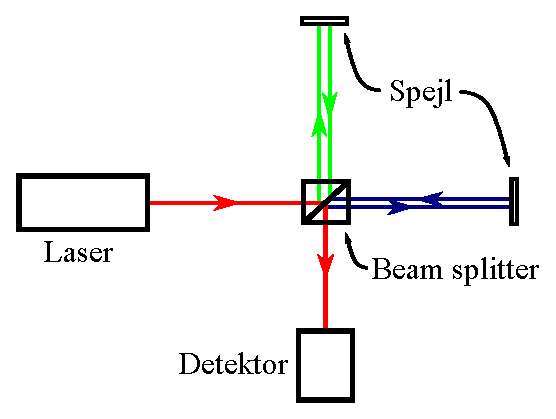
\includegraphics[width=.6\textwidth]{billeder/MichelsonInterferometerGenerelt.eps}
    \caption{\ldots}
    \label{laser:fig:MichelsonInterferometerGenerelt}
\end{figure}

Michelson interferometeret er en af de mest brugte opstillinger til optisk interferometri. Det er blandt andet benyttet i Michelson-Morley eksperimentet, hvor \ldots, og i LIGO\footnote{Laser Interferometer Gravitational-Wave Observatory}, hvor man kan måle forskelle i lysets tilbagelagte vej i de to interferometerarme på ned til $\nicefrac{1}{\num{10000}}$ af bredden af en proton -- hvilken i forvejen er meget lille -- hvilket er grunden til, at LIGO har kunnet måle gravitationsbølger, som er forstyrrelser i rumtiden.

\end{document}